%%=============================================================================
%% Prototype
%%=============================================================================

\chapter{Prototype}
\label{ch:prototype}

\section{Inleiding}

In dit hoofdstuk zullen een aantal van de verschillende ontwerpelementen die zijn toegelicht in de literatuurstudie worden toegevoegd aan het bestaande platform Innerdreams, met als doel gamification te implementeren. De keuze werd gemaakt om gebruikers toe te laten punten en badges te verzamelen en om een scorebord en beloningswinkel toe te voegen. Deze elementen werden gekozen na een brainstormsessie en een kort onderzoek over de verschillende manieren waarop gamification kan worden geïmplementeerd.

\section{Requirements}

Zoals in de inleiding werd vermeld werd gekozen om een puntensysteem te implementeren.  Gebruikers moeten punten kunnen verzamelen door enquêtes in te vullen en te delen. Meer specifiek moet een gebruiker punten kunnen verzamelen per volledig succesvol ingevulde pagina van een enquête en als een enquête volledig wordt voltooid. Punten moeten ook kunnen worden verzameld als een gebruiker de afgelegde enquête deelt en als deze gedeelde enquête succesvol wordt voltooid door de persoon waarmee deze gedeeld werd. Ook moeten gebruikers badges kunnen verzamelen als een mijlpaal wordt bereikt. Hier werd gekozen om het behalen van badges enkel te laten afhangen van het afleggen van enquêtes. Vervolgens moet een gebruiker ook een scorebord kunnen raadplegen waarin de rangschikking, gebruikersnaam en het totaal aantal verzamelde punten van alle gebruikers zal worden weergegeven. Ten slotte moet het mogelijk zijn voor een gebruiker om zijn/haar verzamelde punten te gebruiken in een beloningswinkel om verschillende artikelen aan te schaffen.

\section{Uitwerking}

\subsection{Punten}

Om het puntensysteem uit te werken werd gekozen om gebruikers punten te laten verzamelen bij het invullen en delen van enquêtes. Hiervoor is het nodig dat de mogelijkheid bestaat om aan bepaalde enquêtes punten te gaan toewijzen.

Een eerste noodzakelijke aanpassing was het toevoegen van een tabel aan de SQL databank om de punten die kunnen toegewezen worden aan de verschillende onderdelen van een enquête bij te houden. Zoals te zien is in Figuur \ref{fig:dbdiagram} bestaat de tabel uit de volgende kolommen:

\begin{itemize}
    \item PuntenID: de primaire sleutel om de punten te identificeren.
    \item Pagina: het aantal punten dat wordt verdiend bij het volledig invullen van een pagina van een enquête.
    \item EnqueteCompleted: het aantal punten dat wordt verdiend bij het volledig voltooien van een enquête.
    \item Share: het aantal punten dat wordt verdiend bij het delen van een enquête.
    \item ShareCompleted: het aantal punten dat wordt verdiend bij het succesvol voltooien van een enquête door de persoon met wie de enquête is gedeeld.
    \item EnqueteID: de vreemde sleutel die de punten linkt aan een enquête.
\end{itemize}

\begin{figure}
    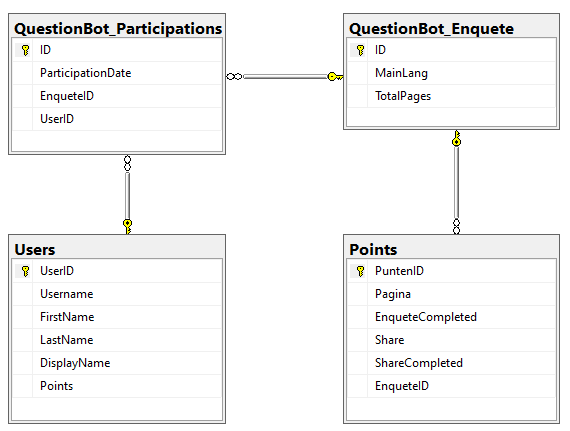
\includegraphics[width=\linewidth]{DBDiagram.png}
    \caption{Het model van de punten.}
    \label{fig:dbdiagram}
\end{figure}

Het was ook nodig om het totale aantal verzamelde punten van iedere individuele gebruiker bij te houden. In Figuur \ref{fig:dbdiagram} is te zien dat aan de gebruikerstabel een extra kolom werd toegevoegd om deze punten vast te hangen aan de gebruikers. Voor zowel gebruikers die een nieuw profiel aanmaken als voor de reeds bestaande gebruikers werd de standaard waarde van hun punten op nul gezet.

Om de punten te kunnen toewijzen aan de verschillende enquêtes werd een nieuwe module aangemaakt. In Figuur \ref{fig:managepoints} is te zien dat in deze module de bestaande enquêtes opgehaald worden en dat de beheerder hierin de respectievelijke punten kan gaan toewijzen aan de enquêtes.

\begin{figure}
    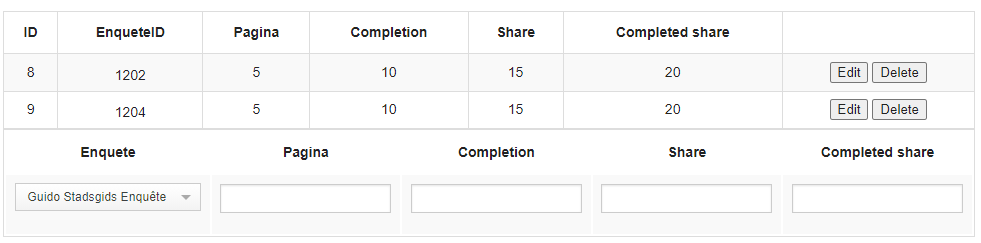
\includegraphics[width=\linewidth]{ManagePoints.png}
    \caption{De beheertool om punten toe te wijzen.}
    \label{fig:managepoints}
\end{figure}

Eenmaal een gebruiker het einde van een enquête bereikt is het nodig om een overzicht van het totale aantal verzamelde punten tijdens het afleggen van de enquête weer te geven. Het is daarom dat werd gekozen om ook een overzichtspagina toe te voegen. Deze pagina verschijnt eenmaal een gebruiker een enquête volledig heeft ingevuld en de inhoud hiervan hangt af van of een enquête punten heeft toegewezen gekregen of niet. Als de enquête punten heeft toegewezen gekregen zal op deze pagina een overzicht worden getoond van de verzamelde punten tijdens het afleggen van de enquête. Op deze pagina is het ook mogelijk om de enquête te gaan delen met andere gebruikers, waardoor nog meer punten kunnen worden verdiend. Als de enquête geen punten heeft toegewezen gekregen zal op dit overzicht een korte bedanking worden getoond.

Soms is het ook mogelijk dat een gebruiker niet moet aangemeld zijn om een enquête in te vullen. Om te zorgen dat de punten die de gebruiker heeft verzameld niet verloren gaan worden deze bijgehouden in zogenaamde sessievariabelen. Een sessievariabele is een object dat voor elke gebruiker apart wordt bijgehouden op de server zolang een sessie tussen de gebruiker en de server actief is. De totale waarde van de verzamelde punten wordt bijgehouden in een sessievariabele tijdens het afleggen van een enquête. Eenmaal de gebruiker op de overzichtspagina terechtkomt en niet aangemeld is wordt de optie gegeven om zich alsnog aan te melden. Als de gebruiker na de doorverwijzing naar de aanmeldpagina terug wordt doorverwezen naar de overzichtspagina zal hij/zij een overzicht zien van de verzamelde punten die bijgehouden zijn in de sessievariabele. Hier krijgt de gebruiker alsnog de kans om de punten te verzilveren.

Als een gebruiker kiest om een enquête te delen zal de URL van de gedeelde enquête een aantal extra parameters bevatten. Een van deze parameters bevat een uniek cijfer dat de gebruiker die de enquête heeft gedeeld zal identificeren. Bij de start van het afleggen van een enquête wordt een controle uitgevoerd om de URL. Als deze URL de eerder vermelde unieke identificatie bevat zullen aan deze gebruiker een aantal vooraf bepaalde punten worden toegewezen. Eenmaal de enquête wordt voltooid zullen aan deze gebruiker opnieuw een aantal punten worden toegewezen.

\subsection{Badges}

Voor het behalen van badges werd gekozen om deze te gaan koppelen aan het totale aantal deelnames van een gebruiker aan enquêtes. Een deelname wordt toegevoegd aan de databank eenmaal een gebruiker tenminste één pagina heeft ingevuld van een enquête.

In figuur \ref{fig:dbbadge} is te zien dat voor het bijhouden van de verschillende badges een extra tabel werd toegevoegd aan de SQL databank. Deze tabel bestaat uit de volgende kolommen:

\begin{itemize}
    \item ID: de primaire sleutel om de badge te identificeren.
    \item ImageLink: een verwijzing naar de afbeelding van de badge.
    \item Title: een titel die de badge beschrijft.
    \item TriggerQuery: een SQL-query die wordt uitgevoerd eenmaal aan een bepaalde voorwaarde voldaan is.
\end{itemize}

\begin{figure}
    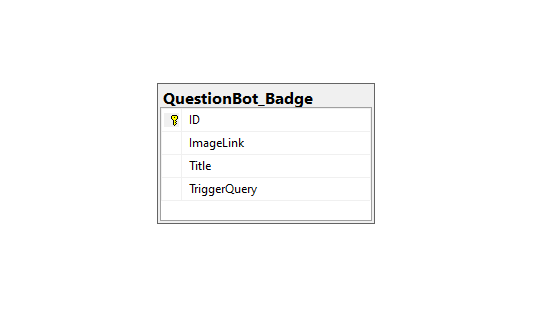
\includegraphics[width=\linewidth]{DBBadge2.png}
    \caption{De badge tabel.}
    \label{fig:dbbadge}
\end{figure}

Wanneer de gebruiker de enquête volledig heeft ingevuld en op de overzichtspagina terechtkomt zullen twee lijsten van badges worden opgehaald. De eerste lijst van badges bestaat uit alle badges die op dat moment aan het systeem zijn toegevoegd. De tweede lijst van badges omvat alle badges die een gebruiker heeft behaald tijdens het invullen van enquêtes. Eenmaal deze twee lijsten zijn opgehaald zullen deze met elkaar worden vergeleken op basis van de unieke identificatie van de badges. Eenmaal een badge wordt tegengekomen die de gebruiker nog niet heeft behaald zal worden gecontroleerd of hij/zij voldoet aan de voorwaarden om deze te behalen. Deze controle zal gebeuren aan de hand van het uitvoeren van een stored procedure, die te zien is in Listing \ref{lst:csb}. In deze stored procedure zal de eerder vermelde trigger query, die gelinkt is aan de desbetreffende badge, worden uitgevoerd.

\begin{lstlisting}[caption={De CheckSucceededBadge stored procedure.},
    label={lst:csb},
    language=SQL,
    showspaces=false,
    basicstyle=\ttfamily,
    numbers=left,
    numberstyle=\tiny,
    numbersep=1pt,
    breaklines=true
    commentstyle=\color{gray}]
    ALTER PROCEDURE [dbo].[QuestionBot_CheckSucceededBadge](@BadgeID int, @UserID int) as
    BEGIN
    Declare @statement as nvarchar(max) 
    set @statement = (select TriggerQuery from QuestionBot_Badge where ID = @BadgeID) 
    EXECUTE sp_executesql @statement , N'@UserID int',@UserID=@UserID
    END
\end{lstlisting}

In Listing \ref{lst:tq} is te zien hoe zo een trigger query er uit ziet en functioneert. Voor een specifieke gebruiker wordt de som van het totale aantal deelnames aan alle enquêtes genomen. Als deze som voldoet aan een bepaalde voorwaarde zal een bit geretourneerd worden. Als deze bit 1 is wil dit zeggen dat de gebruiker aan de voorwaarde voldoet en dat de badge behaald is. Als deze bit op 0 staat is niet aan de voorwaarde voldaan en zal de gebruiker de badge niet krijgen. In dit voorbeeld is te zien dat voor de huidige gebruiker wordt gecontroleerd of hij/zij minstens één deelname heeft aan een enquête. Als aan deze voorwaarde is voldaan zal deze gebruiker een badge verdienen met bijvoorbeeld de tekst ``Vul je eerste enquête in'' (Figuur \ref{fig:badgeunlocked}).

\begin{figure}
    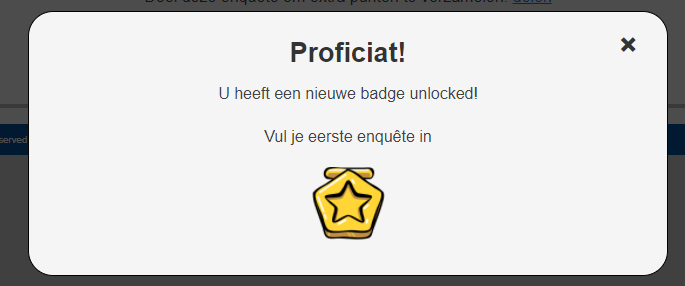
\includegraphics[width=\linewidth]{BadgeUnlocked.png}
    \caption{Het behalen van een badge op Innerdreams.}
    \label{fig:badgeunlocked}
\end{figure}

\begin{lstlisting}[caption={De trigger query van een badge.},
    label={lst:tq},
    language=SQL,
    showspaces=false,
    basicstyle=\ttfamily,
    numbers=left,
    numberstyle=\tiny,
    numbersep=1pt,
    breaklines=true
    commentstyle=\color{gray}]
    declare @Participations int set @Participations = (select count(*) from QuestionBot_Participations where UserID = @UserID) 
    if (@Participations >= 1) select 1 else select 0
\end{lstlisting}

\subsection{Scorebord}

Het scorebord werd ontworpen om respectievelijk de rangschikking, de gebruikersnaam en het totale aantal verzamelde punten van alle gebruikers weer te geven. Om het scorebord te implementeren was het niet nodig om aanpassingen te doen aan de databank. Alle noodzakelijke aanpassingen werden reeds uitgevoerd tijdens het implementeren van de ontwerpelementen in de vorige stappen.

In Listing \ref{lst:gul} is te zien dat gebruik gemaakt werd van een stored procedure, om alle benodigde data van de gebruikers op te halen. In deze stored procedure werd gebruik gemaakt van de \textit{SQL ROW\_NUMBER()} functie. Deze functie zal één of meerdere specifieke kolommen uit een tabel ophalen. Deze kolom(men) kunnen zowel oplopend als aflopend gesorteerd worden. Na het ophalen zal de functie aan elke rij uit de resultatenlijst een unieke, oplopende waarde toewijzen op basis van de geordende kolom. In dit geval haalt de functie een oplopende lijst van de punten van gebruikers op en een lijst van de gebruikersnamen. De functie wijst daarna een waarde toe aan elke rij op basis van de puntenlijst. Deze waarde stelt de rangschikking op het scorebord voor. In het geval dat twee gelijke waarden worden tegengekomen in de lijst van punten wijst de functie de waarde toe op basis van de alfabetische volgorde van de gebruikersnamen. Buiten het ophalen van de rangschikking zal deze stored procedure ook de gebruikersnamen en het totale aantal behaalde punten ophalen van alle gebruikers.

\begin{lstlisting}[caption={De GetUsersLeaderboard stored procedure.},
    label={lst:gul},
    language=SQL,
    showspaces=false,
    basicstyle=\ttfamily,
    numbers=left,
    numberstyle=\tiny,
    numbersep=1pt,
    breaklines=true
    commentstyle=\color{gray}]
    ALTER procedure [dbo].[GetUsersLeaderboard] as
    select ROW_NUMBER() OVER(ORDER BY Points desc, DisplayName) as Rank, DisplayName, Points from dbo.Users
    where IsSuperUser = 0
\end{lstlisting}

Eenmaal de data is opgehaald door de stored procedure zal deze in een overzichtelijke tabel worden weergegeven. In Figuur \ref{fig:leaderboardinnerdreams} is het scorebord zoals het binnen Innerdreams is geïmplementeerd te zien. Binnen dit scorebord kan worden gesorteerd en gefilterd. Sorteren kan gebeuren zowel op de rangschikking, de gebruikersnaam als het aantal behaalde punten en filteren kan gebeuren op de gebruikersnaam. Initeel zal het scorebord alle gebruikers weergeven maar de keuze kan ook gemaakt worden om enkel de top vijf van alle gebruikers met het meeste aantal punten weer te geven.

\begin{figure}
    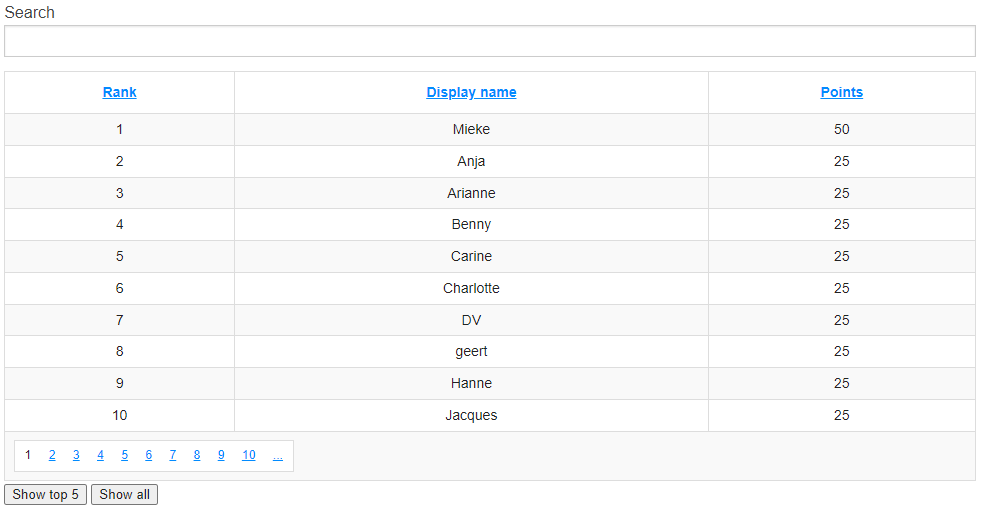
\includegraphics[width=\linewidth]{LeaderboardInnerdreams.png}
    \caption{Het scorebord op Innerdreams.}
    \label{fig:leaderboardinnerdreams}
\end{figure}

\subsection{Beloningswinkel}

Om de punten die de gebruikers hebben verzameld tijdens het afleggen van de verschillende enquêtes niet verloren te laten gaan is het nodig dat deze punten ergens gespendeerd kunnen worden. Het is daarom dat als laatste ontwerpelement werd gekozen om een beloningswinkel te ontwerpen en te gaan implementeren. In deze winkel is het mogelijk om met de verzamelde punten een grote verscheidenheid aan artikelen aan te schaffen.

Om te beginnen met de beloningswinkel te implementeren waren opnieuw een aantal aanpassingen nodig aan de SQL databank. In Figuur \ref{fig:dbdiagramreward} is te zien dat het ten eerste nodig was om een nieuwe tabel toe te voegen waarin de beloningen zelf worden bijgehouden. Deze tabel bestaat uit de volgende kolommen:

\begin{itemize}
    \item RewardID: de primaire sleutel om de beloning te identificeren.
    \item Titel: de titel van de beloning.
    \item Beschrijving: een korte tekst die de beloning beschrijft.
    \item Stock: de hoeveelheid beschikbare beloningen.
    \item Prijs: hoeveel punten nodig zijn om een beloning aan te schaffen.
    \item Startdatum: de datum waarop een beloning actief wordt.
    \item Einddatum: de datum waarop een beloning niet langer actief is.
    \item AantalClaimed: de hoeveelheid beloningen die al aangeschaft zijn.
    \item LeverbaarIn: de landen waarin de beloning beschikbaar is.
    \item ImageLink: een verwijzing naar de afbeelding van de beloning.
    \item AantalPerPersoon: hoeveel beloningen één persoon kan aanschaffen.
    \item VerplichteEnquetes: welke enquêtes verplicht moeten worden voltooid.
    \item Mail: e-mail die wordt verstuurd naar de gebruiker eenmaal een beloning is aangeschaft.
\end{itemize}

\begin{figure}
    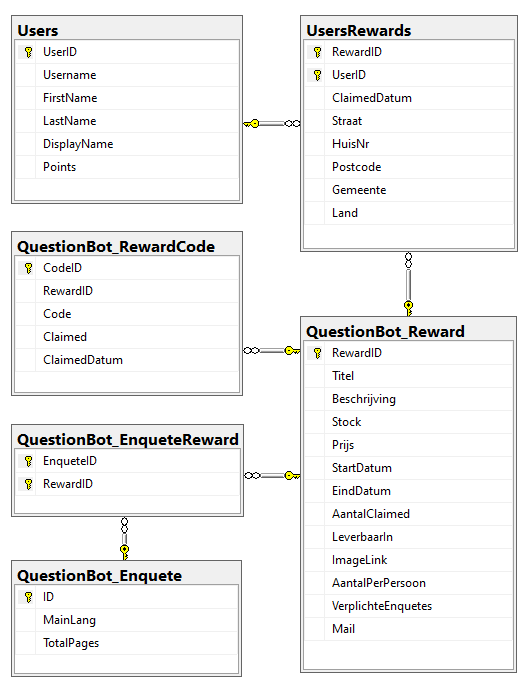
\includegraphics[width=\linewidth]{DBDiagramReward.png}
    \caption{Het model van de beloningen.}
    \label{fig:dbdiagramreward}
\end{figure}

Om een beloning aan te kopen kan ook gebruik gemaakt worden van een beloningscode. De informatie over deze codes wordt bijgehouden in een tabel en hiervoor was het opnieuw nodig om een tabel toe te voegen aan de SQL databank. In Figuur \ref{fig:dbdiagramreward} is de tabel te zien en deze bestaat uit de volgende kolommen:

\begin{itemize}
    \item CodeID: de primaire sleutel om de code te identificeren.
    \item RewardID: de vreemde sleutel die de codes linkt aan een beloning.
    \item Code: de code die gebruikt kan worden om een beloning aan te schaffen.
    \item Claimed: een controle of de code al gebruikt is of niet.
    \item ClaimedDatum: de datum waarop de code is gebruikt.
\end{itemize}

Een beloning zal vaak niet zomaar kunnen worden aangeschaft. Een gebruiker zal één of meerdere enquêtes verplicht moeten voltooien voordat hij/zij in aanmerking komt om de beloning aan te kopen. Het is ook belangrijk om bij te houden waar een beloning beschikbaar is. Dit omdat ze niet altijd beschikbaar zullen zijn in sommige landen.

In Figuur \ref{fig:rewardshop} is te zien hoe de beloningswinkel op Innerdreams eruit ziet. In dit voorbeeld heeft de beloning een kost van 5 punten.

\begin{figure}
    \includegraphics[scale=0.95]{RewardShop.png}
    \centering
    \caption{De beloningswinkel op Innerdreams.}
    \label{fig:rewardshop}
\end{figure}